\subsection{}
What would happen if a tax was introduced into the marketplace?\\
The price the producer receives would be different than the price the consumer pays at equilibrium.\\
\begin{definition}
    \emph{Unit tax} is a fixed amount of tax per unit of the good.\\
    \emph{Ad valorem tax} is a percentage of the price of the good.\\
\end{definition}
\begin{gather}
    t = \text{Unit tax}\\
    P^D = P^S + t\\
    t = P^D - P^S > 0
\end{gather}
Who is paying this tax?\\
\begin{definition}
    {Legal Incidence/Burden} is the person who is legally responsible for paying the tax.\\
    {Economic Incidence/Burden} is the person who actually pays the tax. It is determined by elasticity.\\
\end{definition}
If you are inelastic, you pay more of the tax. If you are elastic, you pay less of the tax.\\
\begin{equation}
    \eta^D < \eta^S \rightarrow \text{Consumers pay more of the tax.}
\end{equation}
\begin{figure}[H]
    \centering
    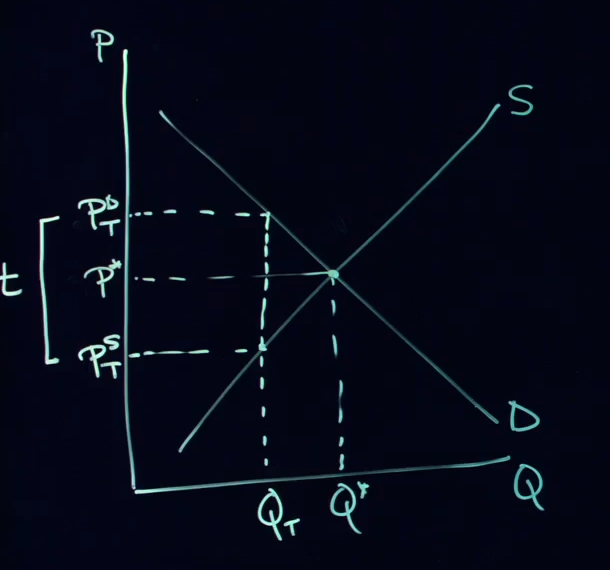
\includegraphics[width=0.5\textwidth]{Chapter4/TaxFiftyFiftyBurden.png}
    \caption{Fifty-Fifty Burden}
\end{figure}
\begin{figure}[H]
    \centering
    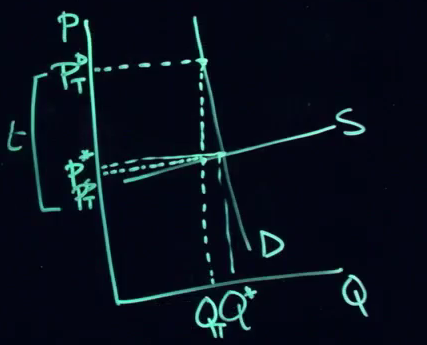
\includegraphics[width=0.5\textwidth]{Chapter4/TaxConsumerBurden.png}
    \caption{Consumer Tax Burden}
\end{figure}